\subsubsection{High Frequency Boost}

This filter was also implemented on top of the FFT filter to boost the high-end
frequencies. The frequencies boosted after approx. 1000 Hz by a factor
of $5\pi$, heuristically determined, and then re-normalized. See Figure \ref{fig:high-boost}.

\begin{figure}
	\centering
	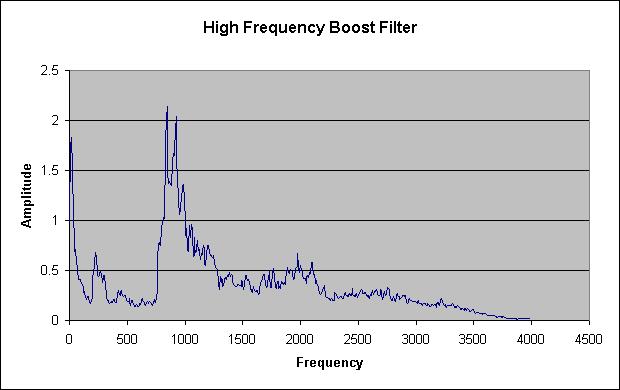
\includegraphics[width=400pt]{../graphics/graphs/high-frequency-boost.png}
	\caption{High frequency boost filter applied to aihua5.wav.}
	\label{fig:high-boost}
\end{figure}
